\documentclass[crop,tikz]{standalone}% 'crop' is the default for v1.0, before it was 'preview'
%\usetikzlibrary{...}% tikz package already loaded by 'tikz' option
\begin{document}
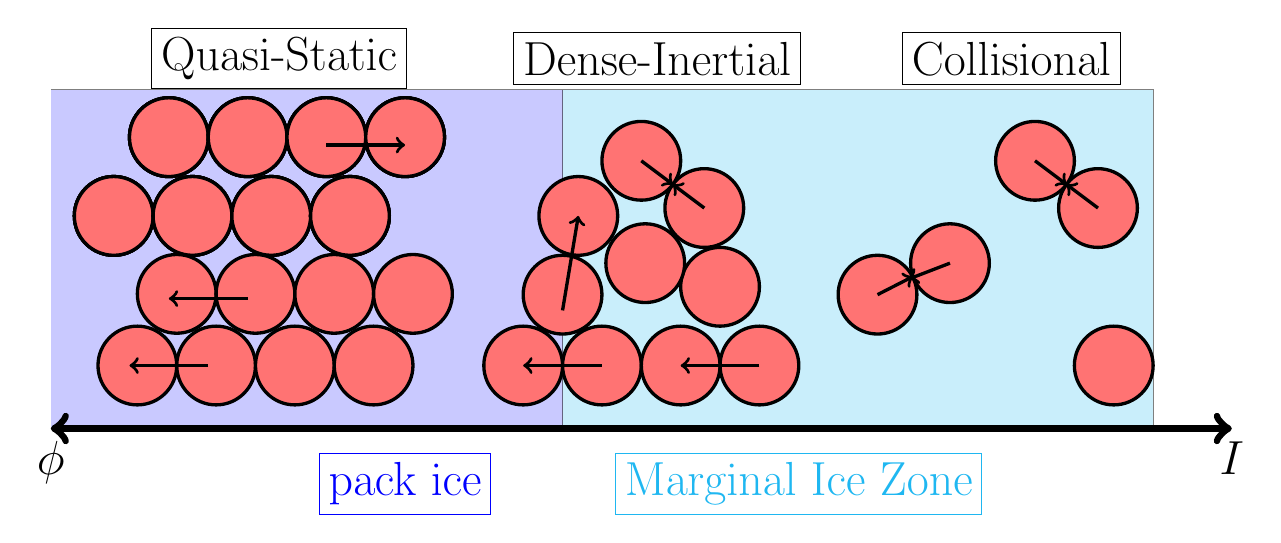
\begin{tikzpicture}[scale = 1]


    \def \b {0};
    \def \c {0.1};
    \def \d {0.1};
    \def \r {2.3};

    \draw[fill=blue!42, opacity = 0.5] (0,-0.5) -- (6.5, -0.5) -- (6.5,3.8) -- (0,3.8 );

    \draw[fill=cyan!42, opacity = 0.5] (6.5, -0.5) -- (14, -0.5) -- (14,3.8) -- (6.5,3.8 );

    \node[draw] at  (2.9, 4.2) { \LARGE Quasi-Static};
    % \node[draw] at (-4,2.7-3.7) { \LARGE Collision};

    \foreach \x in {1, ..., 4}
            \draw [color=black, fill=red!55,very thick] (\x + \b+0.1, 0.3) circle (0.5);

        \foreach \x in {1.5, ..., 4.5}
            \draw [color=black, fill=red!55, very thick] (\x + \b+0.1, 1.21) circle (0.5);

    \foreach \x in {1, ..., 4}
        \foreach \y in {1.5, ..., 4.5}
            \draw [color=black, fill=red!55,very thick] (\x + \b-0.2, 2.2) circle (0.5);


    \foreach \x in {1.5, ..., 4.5}
        \foreach \y in {1.5, ..., 4.5}
            \draw [color=black, fill=red!55,very thick] (\x + \b, 3.2) circle (0.5);

        

    \draw [very thick, ->] (3.5 + \b, 3.1) -- ( 3.5+ \b + 1 , 3.1);
    
    \draw [very thick, ->] (2.5 + \b, 1.15) -- ( 2.5+ \b -1  , 1.15);

    \draw [very thick, ->] (2. + \b, 0.3) -- ( 2.+ \b -1  , 0.3);


    \def \b {5};
    \def \c {0.1};
    \def \d {0.1};
    \def \r {2.3};


    \node[draw] at  (2.7+\b, 4.2) { \LARGE Dense-Inertial};
    % \node[draw] at (-4,2.7-3.7) { \LARGE Collision};

    \foreach \x in {1, ..., 4}
            \draw [color=black, fill=red!55,very thick] (\x + \b, 0.3) circle (0.5);

    % \foreach \x in {1.5, ..., 3.5}
    %         \draw [color=black, fill=red!55, very thick] (\x + \b, 1.3) circle (0.5);
            
    \draw [color=black, fill=red!55, very thick] (1.5 + \b, 1.2) circle (0.5);       
    \draw [color=black, fill=red!55, very thick] (3.5 + \b, 1.3) circle (0.5);  
    \draw [color=black, fill=red!55, very thick] (2.55 + \b, 1.6) circle (0.5);
    \draw [color=black, fill=red!55, very thick] (3.3 + \b, 2.3) circle (0.5);
    \draw [color=black, fill=red!55, very thick] (1.7 + \b, 2.2) circle (0.5);
    \draw [color=black, fill=red!55, very thick] (2.5 + \b, 2.9) circle (0.5);


        
    \draw [very thick, ->] (2.5 + \b, 2.9) -- (2.9 + \b, 2.6);
    \draw [very thick, ->] (3.3 + \b, 2.3) -- (2.9 + \b, 2.6);
    
   \draw [very thick, ->] (1.5 + \b, 1.) -- (1.7 + \b, 2.2);

    \draw [very thick, ->] (2. + \b, 0.3) -- ( 2.+ \b -1  , 0.3);
    \draw [very thick, ->] (4. + \b, 0.3) -- ( 4.+ \b -1  , 0.3);


    \def \b {10};
    \def \c {0.1};
    \def \d {0.1};
    \def \r {2.3};


    \node[draw] at  (2.2+\b, 4.2) { \LARGE Collisional};
            
    \draw [color=black, fill=red!55, very thick] (.5 + \b, 1.2) circle (0.5);    
    \draw [color=black, fill=red!55, very thick] (1.42 + \b, 1.6) circle (0.5);
    \draw [color=black, fill=red!55, very thick] (3.5 + \b, 0.3) circle (0.5);  
    \draw [color=black, fill=red!55, very thick] (3.3 + \b, 2.3) circle (0.5);
    \draw [color=black, fill=red!55, very thick] (2.5 + \b, 2.9) circle (0.5);


        
    \draw [very thick, ->] (2.5 + \b, 2.9) -- (2.9 + \b, 2.6);
    \draw [very thick, ->] (3.3 + \b, 2.3) -- (2.9 + \b, 2.6);

    \draw [very thick, ->] (.5 + \b, 1.2) -- (0.95 + \b, 1.43);
    \draw [very thick, ->] (1.42 + \b, 1.6) -- (0.9 + \b, 1.4);

    \draw [very thick, line width = 1mm, <->] (0 , -0.5) node[below] {\LARGE $\phi$} -- (15, -0.5) node[below] {\LARGE $I$};


    \node[draw, color = blue] at (4.5, -1.2) {\LARGE pack ice};


    \node[draw, color = cyan!88] at (9.5, -1.2) {\LARGE{Marginal Ice Zone}};
\end{tikzpicture}
\end{document}